
\documentclass[letterpaper,hide notes,xcolor={table,svgnames},pdftex,10pt]{beamer}
\def\showexamples{t}


%\usepackage[svgnames]{xcolor}

%% Demo talk
%\documentclass[letterpaper,notes=show]{beamer}

\usecolortheme{crane}
\setbeamertemplate{navigation symbols}{}

\usetheme{MyPittsburgh}
%\usetheme{Frankfurt}

%\usepackage{tipa}

\usepackage{hyperref}
\usepackage{graphicx,xspace}
\usepackage[normalem]{ulem}
\usepackage{multicol}
\usepackage{amsmath,amssymb,amsthm,graphicx,xspace}
\newcommand\SF[1]{$\bigstar$\footnote{SF: #1}}

\usepackage[default]{sourcesanspro}
\usepackage[T1]{fontenc}
\usepackage[scaled]{beramono}
\usepackage{tikzpagenodes}

\newcounter{tmpnumSlide}
\newcounter{tmpnumNote}


% old question code
%\newcommand\question[1]{{$\bigstar$ \small \onlySlide{2}{#1}}}
% \newcommand\nquestion[1]{\ifdefined \presentationonly \textcircled{?} \fi \note{\par{\Large \textbf{?}} #1}}
% \newcommand\nanswer[1]{\note{\par{\Large \textbf{A}} #1}}


 \newcommand\mnote[1]{%
   \addtocounter{tmpnumSlide}{1}
   \ifdefined\showcues {~\tiny\fbox{\arabic{tmpnumSlide}}}\fi
   \note{\setlength{\parskip}{1ex}\addtocounter{tmpnumNote}{1}\textbf{\Large \arabic{tmpnumNote}:} {#1\par}}}

\newcommand\mmnote[1]{\note{\setlength{\parskip}{1ex}#1\par}}

%\newcommand\mnote[2][]{\ifdefined\handoutwithnotes {~\tiny\fbox{#1}}\fi
% \note{\setlength{\parskip}{1ex}\textbf{\Large #1:} #2\par}}

%\newcommand\mnote[2][]{{\tiny\fbox{#1}} \note{\setlength{\parskip}{1ex}\textbf{\Large #1:} #2\par}}

\newcommand\mquestion[2]{{~\color{red}\fbox{?}}\note{\setlength{\parskip}{1ex}\par{\Large \textbf{?}} #1} \note{\setlength{\parskip}{1ex}\par{\Large \textbf{A}} #2\par}\ifdefined \presentationonly \pause \fi}

\newcommand\blackboard[1]{%
\ifdefined   \showblackboard
  {#1}
  \else {\begin{center} \fbox{\colorbox{blue!30}{%
         \begin{minipage}{.95\linewidth}%
           \hspace{\stretch{1}} Some space intentionally left blank; done at the blackboard.%
         \end{minipage}}}\end{center}}%
         \fi%
}



%\newcommand\q{\tikz \node[thick,color=black,shape=circle]{?};}
%\newcommand\q{\ifdefined \presentationonly \textcircled{?} \fi}

\usepackage{listings}
\lstset{basicstyle=\footnotesize\ttfamily,
	breaklines=true,
	aboveskip=15pt,
  	belowskip=15pt,
	frame=lines,
	numbers=left, basicstyle=\scriptsize, numberstyle=\tiny, stepnumber=0, numbersep=2pt
}

\usepackage{siunitx}
\newcommand\sius[1]{\num[group-separator = {,}]{#1}\si{\micro\second}}
\newcommand\sims[1]{\num[group-separator = {,}]{#1}\si{\milli\second}}
\newcommand\sins[1]{\num[group-separator = {,}]{#1}\si{\nano\second}}
\sisetup{group-separator = {,}, group-digits = true}

%% -------------------- tikz --------------------
\usepackage{tikz}
\usetikzlibrary{positioning}
\usetikzlibrary{arrows,backgrounds,automata,decorations.shapes,decorations.pathmorphing,decorations.markings,decorations.text,decorations.pathreplacing}

\tikzstyle{place}=[circle,draw=blue!50,fill=blue!20,thick, inner sep=0pt,minimum size=6mm]
\tikzstyle{transition}=[rectangle,draw=black!50,fill=black!20,thick, inner sep=0pt,minimum size=4mm]

\tikzstyle{block}=[rectangle,draw=black, thick, inner sep=5pt]
\tikzstyle{bullet}=[circle,draw=black, fill=black, thin, inner sep=2pt]

\tikzstyle{pre}=[<-,shorten <=1pt,>=stealth',semithick]
\tikzstyle{post}=[->,shorten >=1pt,>=stealth',semithick]
\tikzstyle{bi}=[<->,shorten >=1pt,shorten <=1pt, >=stealth',semithick]

\tikzstyle{mut}=[-,>=stealth',semithick]

\tikzstyle{treereset}=[dashed,->, shorten >=1pt,>=stealth',thin]

\usepackage{ifmtarg}
\usepackage{xifthen}
\makeatletter
% new counter to now which frame it is within the sequence
\newcounter{multiframecounter}
% initialize buffer for previously used frame title
\gdef\lastframetitle{\textit{undefined}}
% new environment for a multi-frame
\newenvironment{multiframe}[1][]{%
\ifthenelse{\isempty{#1}}{%
% if no frame title was set via optional parameter,
% only increase sequence counter by 1
\addtocounter{multiframecounter}{1}%
}{%
% new frame title has been provided, thus
% reset sequence counter to 1 and buffer frame title for later use
\setcounter{multiframecounter}{1}%
\gdef\lastframetitle{#1}%
}%
% start conventional frame environment and
% automatically set frame title followed by sequence counter
\begin{frame}%
\frametitle{\lastframetitle~{\normalfont(\arabic{multiframecounter})}}%
}{%
\end{frame}%
}
\makeatother

\makeatletter
\newdimen\tu@tmpa%
\newdimen\ydiffl%
\newdimen\xdiffl%
\newcommand\ydiff[2]{%
    \coordinate (tmpnamea) at (#1);%
    \coordinate (tmpnameb) at (#2);%
    \pgfextracty{\tu@tmpa}{\pgfpointanchor{tmpnamea}{center}}%
    \pgfextracty{\ydiffl}{\pgfpointanchor{tmpnameb}{center}}%
    \advance\ydiffl by -\tu@tmpa%
}
\newcommand\xdiff[2]{%
    \coordinate (tmpnamea) at (#1);%
    \coordinate (tmpnameb) at (#2);%
    \pgfextractx{\tu@tmpa}{\pgfpointanchor{tmpnamea}{center}}%
    \pgfextractx{\xdiffl}{\pgfpointanchor{tmpnameb}{center}}%
    \advance\xdiffl by -\tu@tmpa%
}
\makeatother
\newcommand{\copyrightbox}[3][r]{%
\begin{tikzpicture}%
\node[inner sep=0pt,minimum size=2em](ciimage){#2};
\usefont{OT1}{phv}{n}{n}\fontsize{4}{4}\selectfont
\ydiff{ciimage.south}{ciimage.north}
\xdiff{ciimage.west}{ciimage.east}
\ifthenelse{\equal{#1}{r}}{%
\node[inner sep=0pt,right=1ex of ciimage.south east,anchor=north west,rotate=90]%
{\raggedleft\color{black!50}\parbox{\the\ydiffl}{\raggedright{}#3}};%
}{%
\ifthenelse{\equal{#1}{l}}{%
\node[inner sep=0pt,right=1ex of ciimage.south west,anchor=south west,rotate=90]%
{\raggedleft\color{black!50}\parbox{\the\ydiffl}{\raggedright{}#3}};%
}{%
\node[inner sep=0pt,below=1ex of ciimage.south west,anchor=north west]%
{\raggedleft\color{black!50}\parbox{\the\xdiffl}{\raggedright{}#3}};%
}
}
\end{tikzpicture}
}


%% --------------------

%\usepackage[excludeor]{everyhook}
%\PushPreHook{par}{\setbox0=\lastbox\llap{MUH}}\box0}

%\vspace*{\stretch{1}

%\setbox0=\lastbox \llap{\textbullet\enskip}\box0}

\setlength{\parskip}{\fill}

\newcommand\noskips{\setlength{\parskip}{1ex}}
\newcommand\doskips{\setlength{\parskip}{\fill}}

\newcommand\xx{\par\vspace*{\stretch{1}}\par}
\newcommand\xxs{\par\vspace*{2ex}\par}
\newcommand\tuple[1]{\langle #1 \rangle}
\newcommand\code[1]{{\sf \footnotesize #1}}
\newcommand\ex[1]{\uline{Example:} \ifdefined \presentationonly \pause \fi
  \ifdefined\showexamples#1\xspace\else{\uline{\hspace*{2cm}}}\fi}

\newcommand\ceil[1]{\lceil #1 \rceil}


\AtBeginSection[]
{
   \begin{frame}
       \frametitle{Outline}
       \tableofcontents[currentsection]
   \end{frame}
}



\pgfdeclarelayer{edgelayer}
\pgfdeclarelayer{nodelayer}
\pgfsetlayers{edgelayer,nodelayer,main}

\tikzstyle{none}=[inner sep=0pt]
\tikzstyle{rn}=[circle,fill=Red,draw=Black,line width=0.8 pt]
\tikzstyle{gn}=[circle,fill=Lime,draw=Black,line width=0.8 pt]
\tikzstyle{yn}=[circle,fill=Yellow,draw=Black,line width=0.8 pt]
\tikzstyle{empty}=[circle,fill=White,draw=Black]
\tikzstyle{bw} = [rectangle, draw, fill=blue!20, 
    text width=4em, text centered, rounded corners, minimum height=2em]
    
    \newcommand{\CcNote}[1]{% longname
	This work is licensed under the \textit{Creative Commons #1 3.0 License}.%
}
\newcommand{\CcImageBy}[1]{%
	\includegraphics[scale=#1]{creative_commons/cc_by_30.pdf}%
}
\newcommand{\CcImageSa}[1]{%
	\includegraphics[scale=#1]{creative_commons/cc_sa_30.pdf}%
}
\newcommand{\CcImageNc}[1]{%
	\includegraphics[scale=#1]{creative_commons/cc_nc_30.pdf}%
}
\newcommand{\CcGroupBySa}[2]{% zoom, gap
	\CcImageBy{#1}\hspace*{#2}\CcImageNc{#1}\hspace*{#2}\CcImageSa{#1}%
}
\newcommand{\CcLongnameByNcSa}{Attribution-NonCommercial-ShareAlike}

\newenvironment{changemargin}[1]{% 
  \begin{list}{}{% 
    \setlength{\topsep}{0pt}% 
    \setlength{\leftmargin}{#1}% 
    \setlength{\rightmargin}{1em}
    \setlength{\listparindent}{\parindent}% 
    \setlength{\itemindent}{\parindent}% 
    \setlength{\parsep}{\parskip}% 
  }% 
  \item[]}{\end{list}} 



\usepackage{soul}

\title{Lecture 27 --- Liar, Liar, Memory Profiling }

\author{Patrick Lam \& Jeff Zarnett \\ \small \texttt{patrick.lam@uwaterloo.ca jzarnett@uwaterloo.ca}}
\institute{Department of Electrical and Computer Engineering \\
  University of Waterloo}
\date{\today}


\begin{document}

\begin{frame}
  \titlepage
 \end{frame}


\part{Liar, Liar}

\begin{frame}
\frametitle{Liar, Liar}

\begin{center}
	
\includegraphics[width=0.75\textwidth]{images/Liar-Liar.jpg}
\end{center}


\end{frame}

\begin{frame}
\frametitle{Sampling Based Profiling}

Let's open with a video that illustrates one of the problems with sampling-based profiling:

\begin{center}
	\url{https://www.youtube.com/watch?v=jQDjJRYmeWg}
\end{center}

Is this fake?

\end{frame}


\begin{frame}
\frametitle{Assumptions}

The main assumptions underlying sampling are that:

Samples are ``random''; and 

The sample distribution approximates the actual time-spent distribution.

\end{frame}


%%%%%%%%%%%%%%%%%%%%%%%%%%%%%%%%%%%%%%%%%%%%%%%%%%%%%%%%%%%%%%%%%%%%%%%%%%%%%%%%
\begin{frame}
  \frametitle{In the Criminal Justice System...}
  
  
    Who can we trust?\\[1em]
    
    \begin{center}
	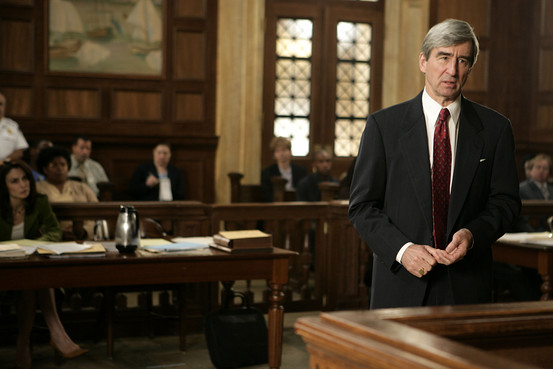
\includegraphics[width=0.6\textwidth]{images/lawandorder.jpg}
	\end{center}
\end{frame}


\part{Lies from Metrics}

%%%%%%%%%%%%%%%%%%%%%%%%%%%%%%%%%%%%%%%%%%%%%%%%%%%%%%%%%%%%%%%%%%%%%%%%%%%%%%%%
\begin{frame}
  \partpage
\end{frame}
%%%%%%%%%%%%%%%%%%%%%%%%%%%%%%%%%%%%%%%%%%%%%%%%%%%%%%%%%%%%%%%%%%%%%%%%%%%%%%%%

%%%%%%%%%%%%%%%%%%%%%%%%%%%%%%%%%%%%%%%%%%%%%%%%%%%%%%%%%%%%%%%%%%%%%%%%%%%%%%%%
\begin{frame}
  \frametitle{Lying perf counters}
  
  
    While app-specific metrics can lie too,\\
    mostly we'll talk about CPU perf counters.
  



  \begin{center}
    Reference: Paul Khuong,\\
  \tiny
  \url{http://www.pvk.ca/Blog/2014/10/19/performance-optimisation-~-writing-an-essay/}

  \end{center}

\end{frame}
%%%%%%%%%%%%%%%%%%%%%%%%%%%%%%%%%%%%%%%%%%%%%%%%%%%%%%%%%%%%%%%%%%%%%%%%%%%%%%%%

%%%%%%%%%%%%%%%%%%%%%%%%%%%%%%%%%%%%%%%%%%%%%%%%%%%%%%%%%%%%%%%%%%%%%%%%%%%%%%%%
\begin{frame}
  \frametitle{mfence}


    We've talked about {\tt mfence}.\\
    Used in spinlocks, for instance.\\[2em]
    Profiles said: spinlocking didn't take much time.\\
    Empirically: eliminating spinlocks = better than expected!
    
  
  
\end{frame}
%%%%%%%%%%%%%%%%%%%%%%%%%%%%%%%%%%%%%%%%%%%%%%%%%%%%%%%%%%%%%%%%%%%%%%%%%%%%%%%%

%%%%%%%%%%%%%%%%%%%%%%%%%%%%%%%%%%%%%%%%%%%%%%%%%%%%%%%%%%%%%%%%%%%%%%%%%%%%%%%%
\begin{frame}
  \frametitle{Exploring the lie}

  
    Next step: create microbenchmarks.\\[1em]
    Memory accesses to uncached locations,\\
    or computations,\\[1em]
    surrounded by store pairs/mfence/locks.\\[1em]
    Use perf to evaluate impact of mfence vs lock.
  

\end{frame}
%%%%%%%%%%%%%%%%%%%%%%%%%%%%%%%%%%%%%%%%%%%%%%%%%%%%%%%%%%%%%%%%%%%%%%%%%%%%%%%%

%%%%%%%%%%%%%%%%%%%%%%%%%%%%%%%%%%%%%%%%%%%%%%%%%%%%%%%%%%%%%%%%%%%%%%%%%%%%%%%%
\begin{frame}[fragile]
  \frametitle{perf for lock}

    \begin{lstlisting}
$ perf annotate -s cache_misses
[...]
    0.06 :        4006b0:       and    %rdx,%r10
    0.00 :        4006b3:       add    $0x1,%r9
    ;; random (out of last level cache) read
    0.00 :        4006b7:       mov    (%rsi,%r10,8),%rbp
   30.37 :        4006bb:       mov    %rcx,%r10
    ;; foo is cached, to simulate our internal lock
    0.12 :        4006be:       mov    %r9,0x200fbb(%rip)
    0.00 :        4006c5:       shl    $0x17,%r10
    [... Skipping arithmetic with < 1% weight in the profile]
    ;; locked increment of an in-cache "lock" byte
    1.00 :        4006e7:       lock incb 0x200d92(%rip)
   21.57 :        4006ee:       add    $0x1,%rax
    [...]
    ;; random out of cache read
    0.00 :        400704:       xor    (%rsi,%r10,8),%rbp
   21.99 :        400708:       xor    %r9,%r8
    [...]
    ;; locked in-cache decrement
    0.00 :        400729:       lock decb 0x200d50(%rip)
   18.61 :        400730:       add    $0x1,%rax
    [...]
    0.92 :        400755:       jne    4006b0 <cache_misses+0x30>
    \end{lstlisting}


\end{frame}
%%%%%%%%%%%%%%%%%%%%%%%%%%%%%%%%%%%%%%%%%%%%%%%%%%%%%%%%%%%%%%%%%%%%%%%%%%%%%%%%

%%%%%%%%%%%%%%%%%%%%%%%%%%%%%%%%%%%%%%%%%%%%%%%%%%%%%%%%%%%%%%%%%%%%%%%%%%%%%%%%
\begin{frame}
  \frametitle{lock's effects}

  
    Reads take 30 + 22 = 52\% of runtime\\
    Locks take 19 + 21 = 40\%.
  

\end{frame}
%%%%%%%%%%%%%%%%%%%%%%%%%%%%%%%%%%%%%%%%%%%%%%%%%%%%%%%%%%%%%%%%%%%%%%%%%%%%%%%%

%%%%%%%%%%%%%%%%%%%%%%%%%%%%%%%%%%%%%%%%%%%%%%%%%%%%%%%%%%%%%%%%%%%%%%%%%%%%%%%%
\begin{frame}[fragile]
  \frametitle{perf for mfence}

  \begin{lstlisting}
$ perf annotate -s cache_misses
[...]
    0.00 :        4006b0:       and    %rdx,%r10
    0.00 :        4006b3:       add    $0x1,%r9
    ;; random read
    0.00 :        4006b7:       mov    (%rsi,%r10,8),%rbp
   42.04 :        4006bb:       mov    %rcx,%r10
    ;; store to cached memory (lock word)
    0.00 :        4006be:       mov    %r9,0x200fbb(%rip)
    [...]
    0.20 :        4006e7:       mfence 
    5.26 :        4006ea:       add    $0x1,%rax
    [...]
    ;; random read
    0.19 :        400700:       xor    (%rsi,%r10,8),%rbp
   43.13 :        400704:       xor    %r9,%r8
    [...]
    0.00 :        400725:       mfence 
    4.96 :        400728:       add    $0x1,%rax
    0.92 :        40072c:       add    $0x1,%rax
    [...]
    0.36 :        40074d:       jne    4006b0 <cache_misses+0x30>
  \end{lstlisting}

\end{frame}
%%%%%%%%%%%%%%%%%%%%%%%%%%%%%%%%%%%%%%%%%%%%%%%%%%%%%%%%%%%%%%%%%%%%%%%%%%%%%%%%

%%%%%%%%%%%%%%%%%%%%%%%%%%%%%%%%%%%%%%%%%%%%%%%%%%%%%%%%%%%%%%%%%%%%%%%%%%%%%%%%
\begin{frame}
  \frametitle{mfence's effects}

  
    Looks like the reads take 85\% of runtime,\\
    while the mfence takes 15\% of runtime.
  

\end{frame}
%%%%%%%%%%%%%%%%%%%%%%%%%%%%%%%%%%%%%%%%%%%%%%%%%%%%%%%%%%%%%%%%%%%%%%%%%%%%%%%%

%%%%%%%%%%%%%%%%%%%%%%%%%%%%%%%%%%%%%%%%%%%%%%%%%%%%%%%%%%%%%%%%%%%%%%%%%%%%%%%%
\begin{frame}
  \frametitle{Bigger picture}

  
    Must also look at total \# of cycles.\\[1em]
    \begin{tabular}{lr}
    No atomic/fence:& 2.81e9 cycles\\
    lock inc/dec: & 3.66e9 cycles\\
    mfence: & 19.60e9 cycles
    \end{tabular}
~\\[1em]
    That 15\% number is a total lie.
  
  \begin{center}
	
\includegraphics[width=0.3\textwidth]{images/maury.jpg}
\end{center}

\end{frame}
%%%%%%%%%%%%%%%%%%%%%%%%%%%%%%%%%%%%%%%%%%%%%%%%%%%%%%%%%%%%%%%%%%%%%%%%%%%%%%%%

%%%%%%%%%%%%%%%%%%%%%%%%%%%%%%%%%%%%%%%%%%%%%%%%%%%%%%%%%%%%%%%%%%%%%%%%%%%%%%%%
\begin{frame}
  \frametitle{Conclusions}

  
    \begin{itemize}
    \item mfence underestimated;
      \item lock overestimated.
    \end{itemize}
    ~\\
    Why? \\[1em]
    mfence = pipeline flush,\\
    costs attributed to instructions being flushed.\\
  

\end{frame}
%%%%%%%%%%%%%%%%%%%%%%%%%%%%%%%%%%%%%%%%%%%%%%%%%%%%%%%%%%%%%%%%%%%%%%%%%%%%%%%%

\part{The Long Tail}

\begin{frame}
\partpage
\end{frame}



\begin{frame}
\frametitle{The Long Tail}

Suppose we have a task that's going to get distributed over multiple computers (like a search). 

If we look at the latency distribution, the problem is mostly that we see a long tail of events. 

When we are doing a computation or search where we need all the results, we can only go as the slowest step.

\end{frame}



\begin{frame}
\frametitle{Grab the Tiger by the Tail}

\begin{center}
	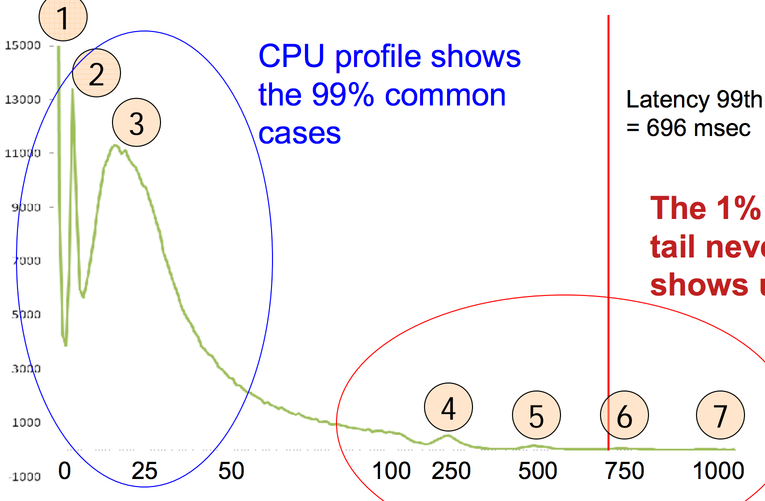
\includegraphics[width=0.85\textwidth]{images/disk_tail.png}
\end{center}

\end{frame}



\begin{frame}
\frametitle{Explaining the Peaks}

\begin{enumerate}
	\item Found in RAM
	\item Disk Cache
	\item Disk
	\item and above... very strange!
\end{enumerate}

\end{frame}



\begin{frame}
\frametitle{Why 250, 500, 750, 1000?}

Answer: CPU throttling!

This was happening on 25\% of disk servers at Google, for an average of half an hour a day!

\end{frame}



\begin{frame}
\frametitle{Faster than a Speeding Bullet}

Another problem with sampling,
this time from Lucene:

\begin{center}
	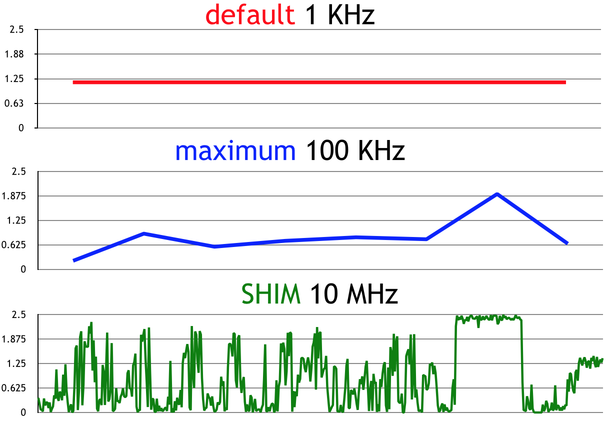
\includegraphics[width=0.7\textwidth]{images/perf-sample.png}
\end{center}

Why is perf limited to 100~KHz?

\end{frame}



\begin{frame}
\frametitle{Processing Interrupts}

Answer: perf samples are done with interrupts (slow). 

If you crank up the rate of interrupts, before long, you are spending all your time handling the interrupts rather than doing useful work.

SHIM gets around this by being more invasive.

This produces a bunch of data which can be dealt with later.

\end{frame}

\part{Lies from Counters}

\begin{frame}
\partpage
\end{frame}


\begin{frame}
\frametitle{Counter This}

Rust compiler hackers were trying to include
support for hardware performance counters (what perf reports).

To make counters as deterministic as possible:
\begin{itemize}
\item disable Address Space Layout Randomization (randomized pointer addresses affect hash layouts);
\item subtract time spent processing interrupts (IRQs);
\item profile one thread only (if you can, in your context).
\end{itemize}


\end{frame}


\begin{frame}
\frametitle{Problem?}

\begin{center}

\includegraphics{images/L27-eb-tweet.png}
\end{center}


\end{frame}



\part{Lies about Calling Context}

%%%%%%%%%%%%%%%%%%%%%%%%%%%%%%%%%%%%%%%%%%%%%%%%%%%%%%%%%%%%%%%%%%%%%%%%%%%%%%%%
\begin{frame}
  \partpage
\end{frame}
%%%%%%%%%%%%%%%%%%%%%%%%%%%%%%%%%%%%%%%%%%%%%%%%%%%%%%%%%%%%%%%%%%%%%%%%%%%%%%%%


\begin{frame}
\frametitle{Profilers, Lying?}

This part is somewhat outdated now, as it's a pretty specific technical problem that especially arises under the {\tt gprof} tool. 

It's still a good example of lying tools, though.

  \begin{center}
    Reference: Yossi Kreinin,\\
  \tiny
  \url{http://www.yosefk.com/blog/how-profilers-lie-the-cases-of-gprof-and-kcachegrind.html}
  \end{center}

\end{frame}
%%%%%%%%%%%%%%%%%%%%%%%%%%%%%%%%%%%%%%%%%%%%%%%%%%%%%%%%%%%%%%%%%%%%%%%%%%%%%%%%

%%%%%%%%%%%%%%%%%%%%%%%%%%%%%%%%%%%%%%%%%%%%%%%%%%%%%%%%%%%%%%%%%%%%%%%%%%%%%%%%
\begin{frame}
\frametitle{gprof said what?}

gprof uses two C standard-library functions: {\bf profil()} and {\bf mcount()}.

\begin{itemize}
\item {\bf profil()}: asks glibc to record which instruction 
  is currently executing (100$\times$/second).
\item {\bf mcount()}: records call graph edges; called by {\tt -pg} instrumentation.
\end{itemize}


  
\end{frame}
%%%%%%%%%%%%%%%%%%%%%%%%%%%%%%%%%%%%%%%%%%%%%%%%%%%%%%%%%%%%%%%%%%%%%%%%%%%%%%%%

%%%%%%%%%%%%%%%%%%%%%%%%%%%%%%%%%%%%%%%%%%%%%%%%%%%%%%%%%%%%%%%%%%%%%%%%%%%%%%%%
\begin{frame}
  \frametitle{Getting it Wrong}

Hence, {\bf profil} information is statistical, while {\bf mcount}
information is exact.  

gprof can draw unreliable inferences. 

If you have a method \texttt{easy} and a method \texttt{hard}, each of which is called once, and \texttt{hard} takes up almost all the CPU time...


gprof might divide total time by 2 and report bogus results.

\end{frame}
%%%%%%%%%%%%%%%%%%%%%%%%%%%%%%%%%%%%%%%%%%%%%%%%%%%%%%%%%%%%%%%%%%%%%%%%%%%%%%%%

%%%%%%%%%%%%%%%%%%%%%%%%%%%%%%%%%%%%%%%%%%%%%%%%%%%%%%%%%%%%%%%%%%%%%%%%%%%%%%%%
\begin{frame}[fragile]
  \frametitle{What's Wrong?}

The following results from gprof are suspect (among others):

\begin{itemize}
  \item contribution of children to parents;
  \item total runtime spent in self+children;
\end{itemize}


When are call graph edges right?
Two cases:

    \begin{itemize}
    \item functions with only one caller
      (e.g. {\tt f()} only called by {\tt g()}); or,
    \item functions which always take the same time to complete
      (e.g. {\tt rand()}).
    \end{itemize}


\end{frame}
%%%%%%%%%%%%%%%%%%%%%%%%%%%%%%%%%%%%%%%%%%%%%%%%%%%%%%%%%%%%%%%%%%%%%%%%%%%%%%%%


\begin{frame}
\frametitle{Other Tools}

Next, we'll talk about callgrind/KCacheGrind.

KCacheGrind is a frontend to callgrind. callgrind gives better information, but imposes more overhead.


KCacheGrind works properly on the earlier hard/easy example, but we can still deceive it with more complicated examples.

\end{frame}


%%%%%%%%%%%%%%%%%%%%%%%%%%%%%%%%%%%%%%%%%%%%%%%%%%%%%%%%%%%%%%%%%%%%%%%%%%%%%%%%
\begin{frame}
  \frametitle{Lies  summary}
  
    Some results are exact;\\
    some results are sampled;\\
    some results are interpolated.\\[1em]

    If you understand the tool, \\
    you understand where it can go wrong.\\[1em]

    Understand your tools!
  
\end{frame}
%%%%%%%%%%%%%%%%%%%%%%%%%%%%%%%%%%%%%%%%%%%%%%%%%%%%%%%%%%%%%%%%%%%%%%%%%%%%%%%%


\part{Memory Profiling}
\begin{frame}
\partpage
\end{frame}

\begin{frame}
\frametitle{\st{Memory Profiling} Return to Asgard}

\large

So far: CPU profiling. 

Memory profiling is also a thing; \\
\qquad specifically heap profiling.

``Still Reachable'': not freed \& still have pointers, \\
\qquad but should have been freed?


\end{frame}



\begin{frame}
\frametitle{\st{Memory Profiling} Return to Asgard}

\large

As with queueing theory:\\
\qquad allocs $>$ frees $\Longrightarrow$ usage $\rightarrow \infty$

At least more paging, maybe total out-of-memory.

But! Memory isn't really lost: we could free it.

Our tool for this comes from the Valgrind tool suite.


\end{frame}


\begin{frame}
\frametitle{DHAT}
DHAT tracks allocation points and what happens to them over a program's execution. 

An allocation point is a point in the program which allocates memory.

\end{frame}


\begin{frame}[fragile]
\frametitle{Leaf Node}

{\scriptsize
\begin{verbatim}
AP 1.1.1.1/2 {
  Total:     31,460,928 bytes (2.32%, 1,565.9/Minstr) in 262,171 blocks (4.41%, 13.05/Minstr), 
     avg size 120 bytes, avg lifetime 986,406,885.05 instrs (4.91% of program duration)
  Max:       16,779,136 bytes in 65,543 blocks, avg size 256 bytes
  At t-gmax: 0 bytes (0%) in 0 blocks (0%), avg size 0 bytes
  At t-end:  0 bytes (0%) in 0 blocks (0%), avg size 0 bytes
  Reads:     5,964,704 bytes (0.11%, 296.88/Minstr), 0.19/byte
  Writes:    10,487,200 bytes (0.51%, 521.98/Minstr), 0.33/byte
  Allocated at {
    ^1: 0x95CACC9: alloc (alloc.rs:72)
      [omitted]
    ^7: 0x95CACC9: parse_token_trees_until_close_delim (tokentrees.rs:27)
    ^8: 0x95CACC9: syntax::parse::lexer::tokentrees::<impl syntax::parse::lexer::
                          StringReader<'a>>::parse_token_tree (tokentrees.rs:81)
    ^9: 0x95CAC39: parse_token_trees_until_close_delim (tokentrees.rs:26)
    ^10: 0x95CAC39: syntax::parse::lexer::tokentrees::<impl syntax::parse::lexer::
                          StringReader<'a>>::parse_token_tree (tokentrees.rs:81)
    #11: 0x95CAC39: parse_token_trees_until_close_delim (tokentrees.rs:26)
    #12: 0x95CAC39: syntax::parse::lexer::tokentrees::<impl syntax::parse::lexer::
                          StringReader<'a>>::parse_token_tree (tokentrees.rs:81)
  }
}
\end{verbatim}
}


\end{frame}


\begin{frame}
\frametitle{Parents}
 Going up the tree, DHAT tells you about all of the allocation points that share a call-stack
prefix. 

The \texttt{\^} before the number indicates that the line is copied from the parent.

A \# indicates that the line is unique to that node.

A sibling of the example above would diverge at the call on line 10.

\end{frame}



\begin{frame}
\frametitle{Shieldmaiden to Thor}

\begin{center}
	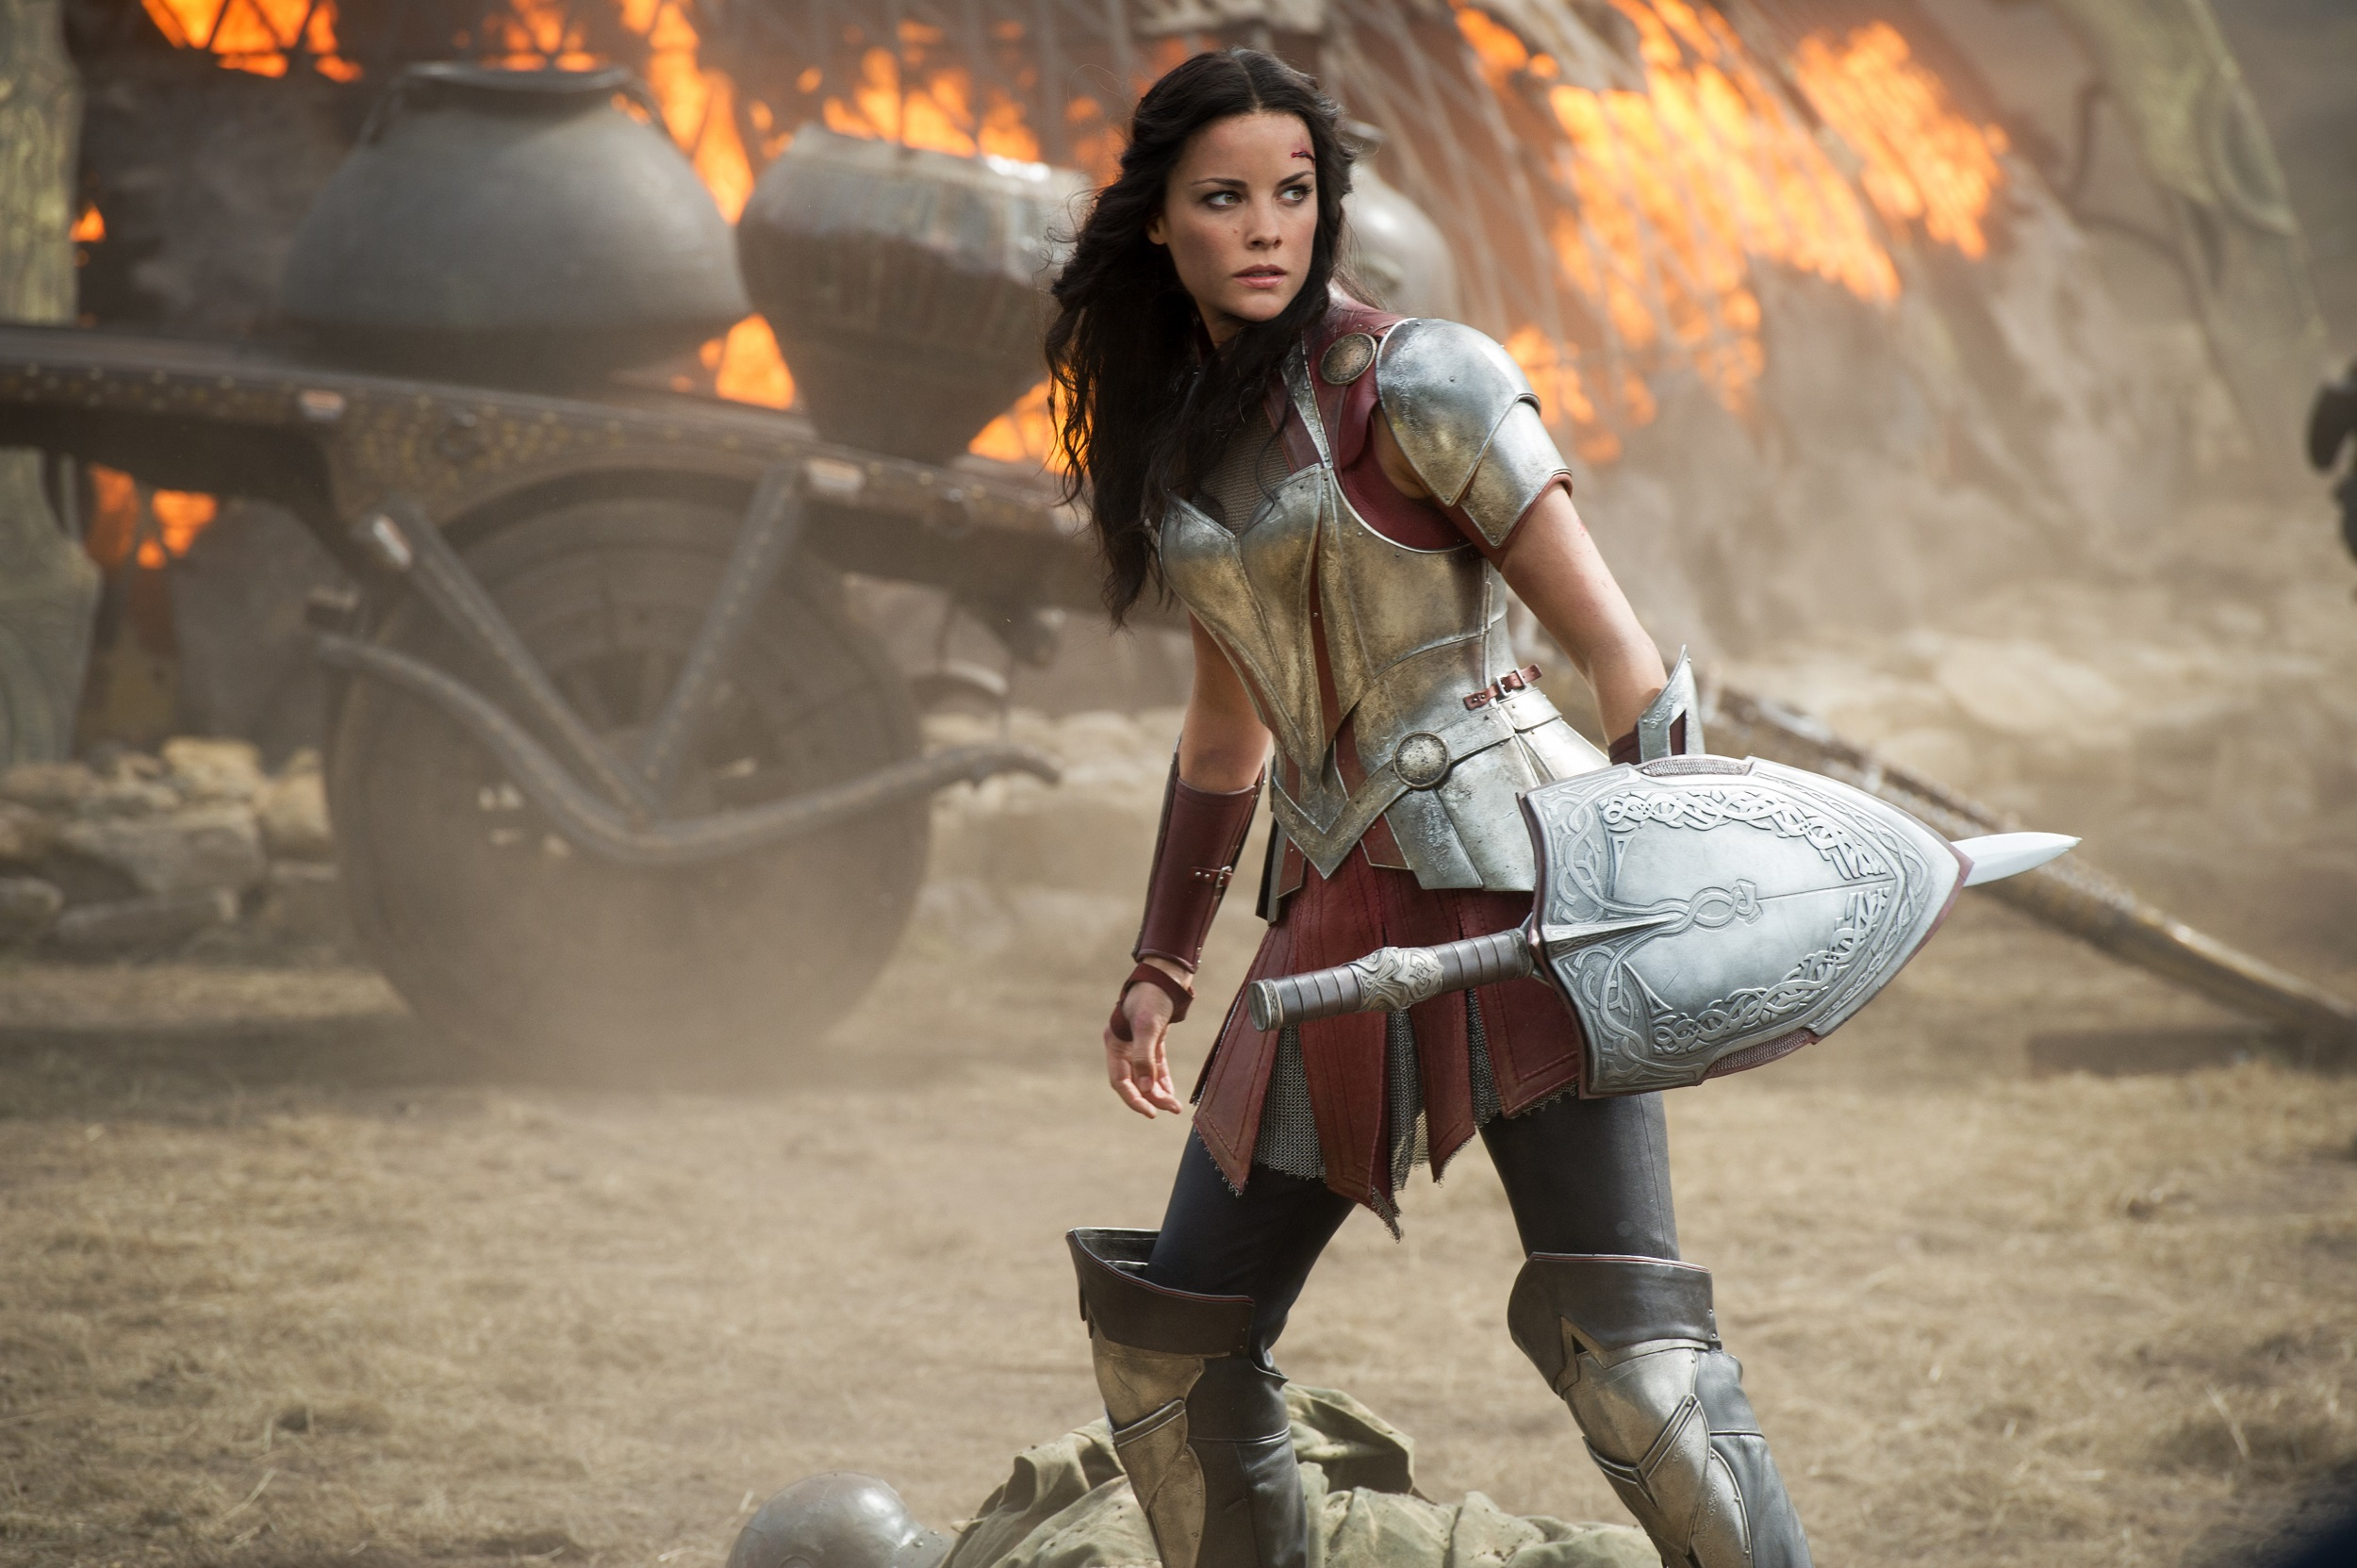
\includegraphics[width=\textwidth]{images/Sif.jpg}
\end{center}

\end{frame}



\begin{frame}
\frametitle{Using Massif}

\Large

What does Massif do? 

\begin{itemize}
\item How much heap memory is your program using?
\item How did this happen?
\end{itemize}

Next up: example from Massif docs.



\end{frame}

\begin{frame}[fragile]
\frametitle{Example Allocation Program}


\begin{lstlisting}[language=Rust]
fn g() {
    let a = Vec::<u8>::with_capacity(4000);
    std::mem::forget(a)
}

fn f() {
    let a = Vec::<u8>::with_capacity(2000);
    std::mem::forget(a);
    g()
}

fn main() {

    let mut a = Vec::with_capacity(10);
    for _i in 0..10 {
	a.push(Box::new([0;1000]))
    }
    f();
    g();
}
\end{lstlisting}

\end{frame}

\begin{frame}[fragile]
\frametitle{Send in Sif}

After we compile, run the command:
{\scriptsize
\begin{verbatim}
plam@amqui ~/c/p/l/l/L/alloc> valgrind --tool=massif target/debug/alloc
==406569== Massif, a heap profiler
==406569== Copyright (C) 2003-2017, and GNU GPL'd, by Nicholas Nethercote
==406569== Using Valgrind-3.16.1 and LibVEX; rerun with -h for copyright info
==406569== Command: target/debug/alloc
==406569== 
==406569== 
\end{verbatim}
}
\end{frame}


\begin{frame}
\frametitle{That Was Useful!!!}

\large

What happened? 

\begin{enumerate}
\item The program ran slowly (because Valgrind!)

\item No summary data on the console \\
\hspace*{2em} (like memcheck or helgrind or cachegrind.)
\end{enumerate}

Weird. What we got instead was the file \texttt{massif.out.[PID]}.


\end{frame}


\begin{frame}
\frametitle{Post-Processing}

\Large

\texttt{massif.out.[PID]}:\\
\hspace*{2cm} plain text, sort of readable.

Better: \texttt{ms\_print}.

Which has nothing whatsoever to do with Microsoft. Promise.


\end{frame}


\begin{frame}[fragile]
\frametitle{Post-Processed Output}
{\scriptsize
\begin{verbatim}

    KB
19.71^                                                                       #
     |                                                                       #
     |                                                                       #
     |                                                                       #
     |                                                                       #
     |                                                                       #
     |                                                                       #
     |                                                                       #
     |                                                                       #
     |                                                                       #
     |                                                                       #
     |                                                                       #
     |                                                                       #
     |                                                                       #
     |                                                                       #
     |                                                                       #
     |                                                                      :#
     |                                                                      :#
     |                                                                      :#
     |                                                                      :#
   0 +----------------------------------------------------------------------->ki
     0                                                                   111.9
\end{verbatim}
}
\end{frame}


\begin{frame}[fragile]
\frametitle{User Friendly, But Not Useful}

\Large

For a long time, nothing happens, then\ldots kaboom! 

Why? We gave it a trivial program.

We should tell Massif to care more \\
about bytes than CPU cycles,\\
with \verb+--time-unit=B+.

Let's try that.



\end{frame}


\begin{frame}
\frametitle{Valgrind (Memcheck) First}


Run valgrind (Memcheck) first and make it happy \\
before we go into figuring out where heap blocks are going with Massif. 

Okay, what to do with the information from Massif, anyway? 

Easy!
\begin{itemize}
\item Start with peak (worst case scenario) \\ and see where that takes you (if anywhere). 

\item You can probably identify some cases where memory is hanging around unnecessarily. 
\end{itemize}



\end{frame}


\begin{frame}
\frametitle{Places to Look with Massif}

\large
Memory usage climbing over a long period of time, perhaps slowly, but never decreasing---memory filling with junk? 

Large spikes in the graph---why so much allocation and deallocation in a short period?
\end{frame}



\begin{frame}[fragile]
\frametitle{Other Massif-ly Useful Things}

\large
\begin{itemize}
	\item stack allocation (\verb+--stacks=yes+).
	\item children of a process \\ (anything split off with \texttt{fork}) if desired.
	\item low level stuff: if going beyond \texttt{malloc}, \texttt{calloc}, \texttt{new}, etc. and using \texttt{mmap} or \texttt{brk} that is usually missed, can do profiling at page level (\verb+--pages-as-heap=yes+).
\end{itemize}

\end{frame}




\begin{frame}
\frametitle{Live Demos}

\large

As is often the case, \\ we have examined the tool on a trivial program. 

Let's see if we can do some\\
 live demos of Massif at work.

\end{frame}


\end{document}


